\documentclass[10pt,a4paper]{article}
\usepackage[T1]{fontenc}
\usepackage[utf8]{inputenc}
\usepackage{lmodern,microtype}
\usepackage[a4paper,margin=22mm,top=25mm,bottom=24mm]{geometry}
\usepackage{amsmath,amssymb,array,booktabs,graphicx,adjustbox,caption,enumitem,fancyhdr,titlesec,xcolor}
\usepackage[colorlinks=true,urlcolor=blue!55!black,linkcolor=black]{hyperref}
\captionsetup{font=small,labelfont=bf,skip=4pt}
\setlist{itemsep=1pt,topsep=3pt,leftmargin=*}
\titlespacing*{\section}{0pt}{12pt}{4pt}
\titlespacing*{\subsection}{0pt}{8pt}{3pt}
\setlength{\parindent}{0pt}\setlength{\parskip}{4pt}
\pagestyle{fancy}\fancyhf{}
\fancyhead[L]{\small Zero-Day SSL Research Report: Label-Scarce Intrusion Detection}
\fancyhead[R]{\small November 2026}
\fancyfoot[C]{\thepage}
\renewcommand{\headrulewidth}{0.4pt}
\begin{document}
\begin{center}{\LARGE\bfseries Self-Supervised Tabular Representation Learning\\ with Decoupled Latent-Centroid Scoring\\ for Zero-Day Intrusion Detection Under Label Scarcity\par}\end{center}
\begin{center}\vspace{-4pt}{\largeTechnical Research Report \& Empirical Validation}\end{center}
\begin{center}\vspace{-6pt}{\smallDate: November 10, 2026 | Status: empirical validation complete | Code and results: \href{https://github.com/AakashBhat1/zeroday-intrusion-detection-ssl}{github.com/AakashBhat1/zeroday-intrusion-detection-ssl}}\end{center}
\vspace{2pt}
\section*{Executive Summary}
Network intrusion detection systems are trained on catalogued attacks and deployed against attacks nobody has labelled yet. Supervised classifiers assign such traffic to a known class with high confidence, and labels for retraining are scarce. This report presents the empirical validation of \textbf{S4\_E06}, a self-supervised tabular model that separates zero-day detection from attack classification. It integrates:

\begin{enumerate}
\item A \textbf{residual tabular encoder} (316,424 parameters) mapping 68 flow statistics to a 128-dimensional latent;
\item \textbf{Dual corrupted views} of every flow, built by marginal feature replacement and Gaussian jitter;
\item A \textbf{multi-task self-supervised objective}: masked feature reconstruction, InfoNCE contrastive learning and a latent hypersphere novelty term;
\item A \textbf{frozen encoder with a lightweight probe} (9,294 parameters) for 14-class triage of known attacks;
\item \textbf{Decoupled zero-day scoring}: the distance of a flow's latent to a fixed centroid, which needs no labels;
\item \textbf{Benign-only threshold calibration} on validation flows, with a 5\% false-alarm target.
\end{enumerate}
The model was benchmarked on CSE-CIC-IDS2018 (16,232,943 flows) against five baselines across four label budgets and ten seeds: 280 runs in total. Training used flows from 14 February to 1 March 2018; the test day, 2 March, contains the Bot family, which appears nowhere in training.

With 10\% of the labels, decoupled scoring reaches a zero-day \textbf{AUROC of 0.9785 $\pm$ 0.0028} and \textbf{AUPRC of 0.9423 $\pm$ 0.0095}. At the calibrated threshold it detects \textbf{98.27\% of Bot flows at a 4.36\% false-positive rate} (F1 0.9700). The next best model, Random Forest, reaches AUROC 0.9528 and detects 58.1\% of Bot flows. All six paired comparisons are statistically significant.

The result has clear limits. With all labels Random Forest matches the proposed model (0.9779), and with 1\% of labels Deep SVDD exceeds it (0.9833). Tree ensembles classify known attacks better at every budget. When known attack families are held out as stand-in zero-days, the decoupled score averages only 0.68 AUROC, so the Bot result does not establish detection of arbitrary new attacks.

\section{Introduction \& Research Problem}
Security operations centres inspect millions of flow records and can label very few of them. A practical detector must work with scarce labels and must flag attack families it was never shown. Existing approaches face four obstacles:

\begin{enumerate}
\item \textbf{Closed-world confidence.} A softmax classifier must place every flow in a known class. Unseen attacks are absorbed into known classes, often with high confidence, so rejection by maximum softmax probability (MSP) is unreliable.
\item \textbf{Label scarcity.} Supervised models degrade as labelled data shrinks, while unlabelled telemetry is abundant and unused.
\item \textbf{One-class models cannot triage.} Detectors trained on benign traffic alone, such as Deep SVDD, flag anomalies but cannot say which known attack a flow belongs to.
\item \textbf{Evaluation leakage.} Random splits let duplicated flows, scalers fitted on all data, or thresholds tuned on test traffic inflate reported numbers.
\end{enumerate}
S4\_E06 addresses these with a decoupled design. A self-supervised encoder learns from unlabelled flows. A small probe on the frozen encoder classifies known attacks. Zero-day detection reads the latent geometry directly, through the distance to a centroid, and never passes through the classifier.

\section{Threat Model \& Evaluation Protocol}
Historical telemetry covers 14 February to 1 March 2018 and contains benign traffic and 13 catalogued attack classes. The locked test set is drawn from 2 March 2018, the only day on which the Bot family (286,191 flows) appears. The last training flow precedes the first test flow by at least 12.0 hours; the source timestamps use a 12-hour clock, so this is a lower bound.

The historical sample caps benign traffic at 108,000 flows and each attack class at 10,000, taking smaller classes whole. It is split 80/20 into training and validation, and validation is split in half (Table 1). Label budgets of 100\%, 10\%, 5\% and 1\% are stratified subsets of the training split: 160,526 / 16,052 / 8,025 / 1,606 flows.

\begin{center}
\captionof{table}{Data partitions.}
\begin{adjustbox}{max width=\linewidth}\small
\begin{tabular}{lll>{\raggedright\arraybackslash}p{7cm}}
\toprule
{\bfseries\boldmath Partition} & {\bfseries\boldmath Source} & {\bfseries\boldmath Flows} & {\bfseries\boldmath Use} \\
\midrule
Training / SSL pool & 14 Feb -- 1 Mar & 160,526 & Pretraining (labels hidden) and label budgets \\
Validation, tuning half & 14 Feb -- 1 Mar & 20,066 & Threshold calibration on its 10,800 benign flows \\
Validation, closed-world half & 14 Feb -- 1 Mar & 20,066 & 14-class accuracy and Macro-F1 \\
Locked test & 2 Mar & 100,000 & 50,000 benign + 50,000 Bot; zero-day metrics \\
\bottomrule
\end{tabular}
\end{adjustbox}
\end{center}
\begin{center}
\captionof{table}{Class composition of the historical sample and the test set.}
\begin{adjustbox}{max width=\linewidth}\small
\begin{tabular}{lll}
\toprule
{\bfseries\boldmath Class} & {\bfseries\boldmath Flows in dataset} & {\bfseries\boldmath Flows sampled} \\
\midrule
Benign & 13,484,708 & 108,000 \\
Brute Force -Web & 611 & 611 \\
Brute Force -XSS & 230 & 230 \\
DDOS attack-HOIC & 686,012 & 10,000 \\
DDOS attack-LOIC-UDP & 1,730 & 1,730 \\
DDoS attacks-LOIC-HTTP & 576,191 & 10,000 \\
DoS attacks-GoldenEye & 41,508 & 10,000 \\
DoS attacks-Hulk & 461,912 & 10,000 \\
DoS attacks-SlowHTTPTest & 139,890 & 10,000 \\
DoS attacks-Slowloris & 10,990 & 10,000 \\
FTP-BruteForce & 193,360 & 10,000 \\
Infilteration & 161,934 & 10,000 \\
SQL Injection & 87 & 87 \\
SSH-Bruteforce & 187,589 & 10,000 \\
Bot (zero-day, test only) & 286,191 & 50,000 \\
\bottomrule
\end{tabular}
\end{adjustbox}
\end{center}
\section{Architecture \& Leakage Safeguards}
\subsection{Data Isolation Protocol}
Every safeguard below is enforced in code before training starts, and the pipeline stops if one fails.

\begin{itemize}
\item \textbf{Train-only pretraining.} The self-supervised pool is the training split with labels hidden. Validation and test flows never reach the encoder.
\item \textbf{Train-only preprocessing.} Median imputation, the robust scaler and the feature selection are fitted on the training split and applied unchanged elsewhere. Scaled features are clipped to $\pm$10.
\item \textbf{Identifier removal.} Destination port, protocol, addresses and timestamps are removed. Eight features that are constant on the training split are dropped, leaving 68 flow statistics.
\item \textbf{Duplicate purging.} Exact duplicate rows are removed before sampling. 32,929 test-day flows whose feature vector also occurs in the historical sample were removed before the test set was drawn, so no test flow has a feature-identical copy in training or validation.
\item \textbf{Validation-only calibration.} Alarm thresholds are set on benign validation flows. Test labels are read only to compute metrics.
\item \textbf{No tuning on the test day.} Hyperparameters were examined on stand-in zero-days built from the historical days (Section 7).
\end{itemize}
One overlap remains and is reported, not removed: 8,881 validation flows share a feature vector with a training flow, because scripted attacks repeat. Closed-world scores are therefore somewhat optimistic for every model alike.

\subsection{Mathematical Formulation}
\textbf{View generation.} For a flow \textit{x} $\in$ $\mathbb{R}$\textsuperscript{68}, two views are produced. Each coordinate is replaced by a draw from that feature's empirical marginal with probability 0.2, and otherwise receives Gaussian jitter:

\begin{equation}
\tilde{x}_{k,j} = m_j \, x^{\mathrm{marg}}_{j} + (1 - m_j)\,(x_j + \epsilon_j), \qquad m_j \sim \mathrm{Bernoulli}(0.2), \quad \epsilon_j \sim \mathcal{N}(0,\ 0.02^{2})
\end{equation}
\textbf{Encoder.} The encoder \textit{f\textsubscript{$\theta$}} applies layer normalisation to the input, projects to 256 dimensions, passes two residual blocks (linear, layer normalisation, GELU, dropout 0.1) and projects to a 128-dimensional latent \textit{z}.

\textbf{Contrastive loss.} A projection head maps each latent to 64 dimensions. The two views of a flow form a positive pair among the 2\textit{N} projections of a batch, with cosine similarity:

\begin{equation}
\mathcal{L}_{\mathrm{con}} = -\frac{1}{2N}\sum_{i=1}^{2N} \log \frac{\exp(\mathrm{sim}(p_i, p_{i^{+}})/\tau_c)}{\sum_{k \neq i} \exp(\mathrm{sim}(p_i, p_k)/\tau_c)}, \qquad \tau_c = 0.1
\end{equation}
\textbf{Masked reconstruction.} A second head predicts the clean features and the corruption mask \textit{m}:

\begin{equation}
\mathcal{L}_{\mathrm{rec}} = \frac{1}{D}\sum_{j=1}^{D} (x_j - \hat{x}_j)^2 + \frac{\gamma}{D}\sum_{j=1}^{D} \mathrm{BCE}(m_j, \hat{m}_j), \qquad \gamma = 1
\end{equation}
\textbf{Hypersphere novelty term.} After five warm-up epochs the centroid \textit{c} is set to the mean latent of the pretraining pool and frozen. For the remaining five epochs latents are pulled toward it:

\begin{equation}
\mathcal{L}_{\mathrm{nov}} = \frac{1}{N}\sum_{i=1}^{N} \| z_i - c \|_2^2, \qquad c = \frac{1}{|\mathcal{D}_{\mathrm{ssl}}|}\sum_{x \in \mathcal{D}_{\mathrm{ssl}}} f_\theta(x) \ \ \mathrm{(fixed\ after\ epoch\ 5)}
\end{equation}
\textbf{Training objective.} Pretraining runs for 10 epochs with AdamW (learning rate 5$\times$10\textsuperscript{$-$4}, batch size 512):

\begin{equation}
\mathcal{L}_{\mathrm{pretrain}} = 0.5\,\mathcal{L}_{\mathrm{rec}} + 0.5\,\mathcal{L}_{\mathrm{con}} + 0.2\,\mathcal{L}_{\mathrm{nov}}
\end{equation}
\textbf{Triage and zero-day scoring.} The encoder is frozen and a probe (128$\rightarrow$64$\rightarrow$14) is trained on the labelled budget with class-weighted cross-entropy. Zero-day detection does not use the probe. A flow is flagged when its distance to the centroid exceeds a threshold calibrated on benign validation flows:

\begin{equation}
S_{\mathrm{nov}}(x^{*}) = \| f_\theta(x^{*}) - c \|_2^2, \qquad \mathrm{alert\ if\ } S_{\mathrm{nov}}(x^{*}) > \tau, \quad \tau = Q_{0.95}\{ S_{\mathrm{nov}}(x) : x \in \mathcal{D}_{\mathrm{val}}^{\mathrm{benign}} \}
\end{equation}
\subsection{Baselines}
\textbf{S4\_E05} uses the same pretraining without the novelty term and then fine-tunes the encoder end to end; it is scored by MSP. \textbf{SCARF} is contrastive pretraining with 60\% feature corruption and a frozen probe. \textbf{Deep SVDD} is a bias-free one-class network trained on the benign flows of each budget. \textbf{Random Forest} (100 trees, depth 15) and \textbf{XGBoost} (100 rounds) are trained on the labelled budget and scored by MSP. Every model is run with seeds 42 to 51.

\section{Empirical Evaluation}
\subsection{Zero-Day Ranking and Closed-World Triage}
Table 3 reports the benchmark at the 10\% budget. Decoupled scoring gives the highest zero-day AUROC and AUPRC, with a seed-to-seed standard deviation of 0.0028, against 0.0207 or more for every baseline. The same encoder scored by MSP is far less reliable, which isolates the gain to the scoring rule. On known attacks the order reverses: the tree ensembles lead, and the proposed model's Macro-F1 is 0.7001 against 0.8493 for XGBoost.

\begin{center}
\captionof{table}{Zero-day detection on the locked test set and closed-world (CW) classification, 10\% labels, 10 seeds (mean $\pm$ sample standard deviation).}
\begin{adjustbox}{max width=\linewidth}\small
\begin{tabular}{lllll}
\toprule
{\bfseries\boldmath Model} & {\bfseries\boldmath Zero-day AUROC} & {\bfseries\boldmath Zero-day AUPRC} & {\bfseries\boldmath CW accuracy} & {\bfseries\boldmath CW Macro-F1} \\
\midrule
{\bfseries\boldmath S4\_E06, decoupled score (proposed)} & {\bfseries\boldmath 0.9785 $\pm$ 0.0028} & {\bfseries\boldmath 0.9423 $\pm$ 0.0095} & {\bfseries\boldmath 0.8813 $\pm$ 0.0131} & {\bfseries\boldmath 0.7001 $\pm$ 0.0234} \\
S4\_E06, MSP score & 0.8747 $\pm$ 0.0822 & 0.7950 $\pm$ 0.1136 & 0.8813 $\pm$ 0.0131 & 0.7001 $\pm$ 0.0234 \\
S4\_E05 (end-to-end fine-tuning) & 0.8818 $\pm$ 0.1086 & 0.8739 $\pm$ 0.0896 & 0.8935 $\pm$ 0.0061 & 0.7471 $\pm$ 0.0103 \\
Random Forest & 0.9528 $\pm$ 0.0207 & 0.9376 $\pm$ 0.0261 & 0.9225 $\pm$ 0.0007 & 0.8267 $\pm$ 0.0152 \\
XGBoost & 0.8352 $\pm$ 0.0946 & 0.7938 $\pm$ 0.1217 & 0.9243 $\pm$ 0.0007 & 0.8493 $\pm$ 0.0161 \\
Deep SVDD & 0.7993 $\pm$ 0.0277 & 0.8152 $\pm$ 0.0220 & N/A & N/A \\
SCARF & 0.4672 $\pm$ 0.0933 & 0.6066 $\pm$ 0.1103 & 0.8619 $\pm$ 0.0133 & 0.6869 $\pm$ 0.0250 \\
\bottomrule
\end{tabular}
\end{adjustbox}
\end{center}
\subsection{Operation at a Calibrated Threshold}
Ranking metrics do not say what an analyst sees. Table 4 fixes each model's threshold at the 95th percentile of its score on benign validation flows and reports the outcome on the test day. All models hold close to the 5\% false-alarm target. The proposed model detects 98.3\% of Bot flows; no baseline exceeds 58\%, and most vary widely between seeds. For seed 42 the threshold $\tau$ = 0.7713 yields 49,033 true positives and 2,182 false positives out of 50,000 flows each.

\begin{center}
\captionof{table}{Operational zero-day detection at the benign-calibrated threshold, 10\% labels, 10 seeds.}
\begin{adjustbox}{max width=\linewidth}\small
\begin{tabular}{llllll}
\toprule
{\bfseries\boldmath Model} & {\bfseries\boldmath $\tau$} & {\bfseries\boldmath Precision} & {\bfseries\boldmath Recall (Bot)} & {\bfseries\boldmath FPR} & {\bfseries\boldmath F1} \\
\midrule
{\bfseries\boldmath S4\_E06, decoupled score (proposed)} & {\bfseries\boldmath 0.7300} & {\bfseries\boldmath 0.9575 $\pm$ 0.0013} & {\bfseries\boldmath 0.9827 $\pm$ 0.0037} & {\bfseries\boldmath 0.0436 $\pm$ 0.0013} & {\bfseries\boldmath 0.9700 $\pm$ 0.0023} \\
S4\_E06, MSP score & 0.5366 & 0.5062 $\pm$ 0.4349 & 0.2230 $\pm$ 0.2554 & 0.0451 $\pm$ 0.0172 & 0.2935 $\pm$ 0.3226 \\
S4\_E05 (end-to-end fine-tuning) & 0.4187 & 0.9453 $\pm$ 0.0215 & 0.4892 $\pm$ 0.2030 & 0.0256 $\pm$ 0.0082 & 0.6259 $\pm$ 0.1667 \\
Random Forest & 0.2293 & 0.9045 $\pm$ 0.0366 & 0.5809 $\pm$ 0.2426 & 0.0529 $\pm$ 0.0071 & 0.6854 $\pm$ 0.1933 \\
XGBoost & 0.2110 & 0.8316 $\pm$ 0.1310 & 0.4561 $\pm$ 0.3128 & 0.0535 $\pm$ 0.0038 & 0.5496 $\pm$ 0.2970 \\
Deep SVDD & 0.0190 & 0.9041 $\pm$ 0.0037 & 0.5095 $\pm$ 0.0041 & 0.0541 $\pm$ 0.0023 & 0.6517 $\pm$ 0.0037 \\
SCARF & 0.5446 & 0.5797 $\pm$ 0.4240 & 0.2756 $\pm$ 0.2394 & 0.0537 $\pm$ 0.0167 & 0.3651 $\pm$ 0.3089 \\
\bottomrule
\end{tabular}
\end{adjustbox}
\end{center}
\subsection{Label-Budget Trajectory}
Table 5 varies the label budget. The decoupled score uses no labels, so it is identical at every budget by construction; only the probe changes. Random Forest improves steadily with labels and matches the proposed model at 100\%. Deep SVDD moves the other way: it is the best detector at 1\% and falls to 0.7224 at 100\%. The proposed model is the best detector at 10\% and 5\%.

\begin{center}
\captionof{table}{Zero-day AUROC by label budget, 10 seeds.}
\begin{adjustbox}{max width=\linewidth}\small
\begin{tabular}{lllll}
\toprule
{\bfseries\boldmath Model} & {\bfseries\boldmath 100\% labels} & {\bfseries\boldmath 10\% labels} & {\bfseries\boldmath 5\% labels} & {\bfseries\boldmath 1\% labels} \\
\midrule
{\bfseries\boldmath S4\_E06, decoupled score (proposed)} & {\bfseries\boldmath 0.9785 $\pm$ 0.0028} & {\bfseries\boldmath 0.9785 $\pm$ 0.0028} & {\bfseries\boldmath 0.9785 $\pm$ 0.0028} & {\bfseries\boldmath 0.9785 $\pm$ 0.0028} \\
S4\_E06, MSP score & 0.8931 $\pm$ 0.1003 & 0.8747 $\pm$ 0.0822 & 0.8487 $\pm$ 0.0699 & 0.8320 $\pm$ 0.0925 \\
S4\_E05 (end-to-end fine-tuning) & 0.9154 $\pm$ 0.0794 & 0.8818 $\pm$ 0.1086 & 0.9033 $\pm$ 0.1018 & 0.8254 $\pm$ 0.0791 \\
Random Forest & 0.9779 $\pm$ 0.0077 & 0.9528 $\pm$ 0.0207 & 0.9359 $\pm$ 0.0215 & 0.8512 $\pm$ 0.0669 \\
XGBoost & 0.9439 $\pm$ 0.0000 & 0.8352 $\pm$ 0.0946 & 0.7702 $\pm$ 0.0939 & 0.8161 $\pm$ 0.1258 \\
Deep SVDD & 0.7224 $\pm$ 0.0922 & 0.7993 $\pm$ 0.0277 & 0.8348 $\pm$ 0.0322 & 0.9833 $\pm$ 0.0045 \\
SCARF & 0.6852 $\pm$ 0.1183 & 0.4672 $\pm$ 0.0933 & 0.4577 $\pm$ 0.1070 & 0.8044 $\pm$ 0.0585 \\
\bottomrule
\end{tabular}
\end{adjustbox}
\end{center}
\begin{center}
\captionof{table}{Closed-world Macro-F1 by label budget (mean of 10 seeds).}
\begin{adjustbox}{max width=\linewidth}\small
\begin{tabular}{lllll}
\toprule
{\bfseries\boldmath Model} & {\bfseries\boldmath 100\% labels} & {\bfseries\boldmath 10\% labels} & {\bfseries\boldmath 5\% labels} & {\bfseries\boldmath 1\% labels} \\
\midrule
S4\_E06 (proposed) & 0.7309 & 0.7001 & 0.6441 & 0.4176 \\
S4\_E05 (end-to-end fine-tuning) & 0.7713 & 0.7471 & 0.7197 & 0.6460 \\
Random Forest & 0.8561 & 0.8267 & 0.8052 & 0.7587 \\
XGBoost & 0.8880 & 0.8493 & 0.8231 & 0.7551 \\
SCARF & 0.7321 & 0.6869 & 0.6209 & 0.4774 \\
\bottomrule
\end{tabular}
\end{adjustbox}
\end{center}
\subsection{Statistical Hypothesis Testing}
Each baseline is compared with the proposed model on seed-paired AUROC using an exact two-sided Wilcoxon signed-rank test (n = 10), with Benjamini--Hochberg correction over the six comparisons and Cliff's $\delta$ as effect size. All six differences are significant at $\alpha$ = 0.05 (Table 7). With ten pairs the smallest attainable raw p-value is 0.0020.

\begin{center}
\captionof{table}{Paired significance tests on zero-day AUROC, 10\% labels.}
\begin{adjustbox}{max width=\linewidth}\small
\begin{tabular}{llllll}
\toprule
{\bfseries\boldmath Proposed vs} & {\bfseries\boldmath Mean $\Delta$AUROC} & {\bfseries\boldmath W} & {\bfseries\boldmath Raw p} & {\bfseries\boldmath BH-adjusted p} & {\bfseries\boldmath Cliff's $\delta$} \\
\midrule
S4\_E06, MSP score & +0.1039 & 0 & 0.0020 & 0.0029 & +0.98 (Large) \\
S4\_E05 (end-to-end fine-tuning) & +0.0967 & 1 & 0.0039 & 0.0039 & +0.80 (Large) \\
Random Forest & +0.0257 & 1 & 0.0039 & 0.0039 & +0.78 (Large) \\
XGBoost & +0.1433 & 0 & 0.0020 & 0.0029 & +1.00 (Large) \\
Deep SVDD & +0.1792 & 0 & 0.0020 & 0.0029 & +1.00 (Large) \\
SCARF & +0.5114 & 0 & 0.0020 & 0.0029 & +1.00 (Large) \\
\bottomrule
\end{tabular}
\end{adjustbox}
\end{center}
\section{Visual Experimental Results}
\begin{center}
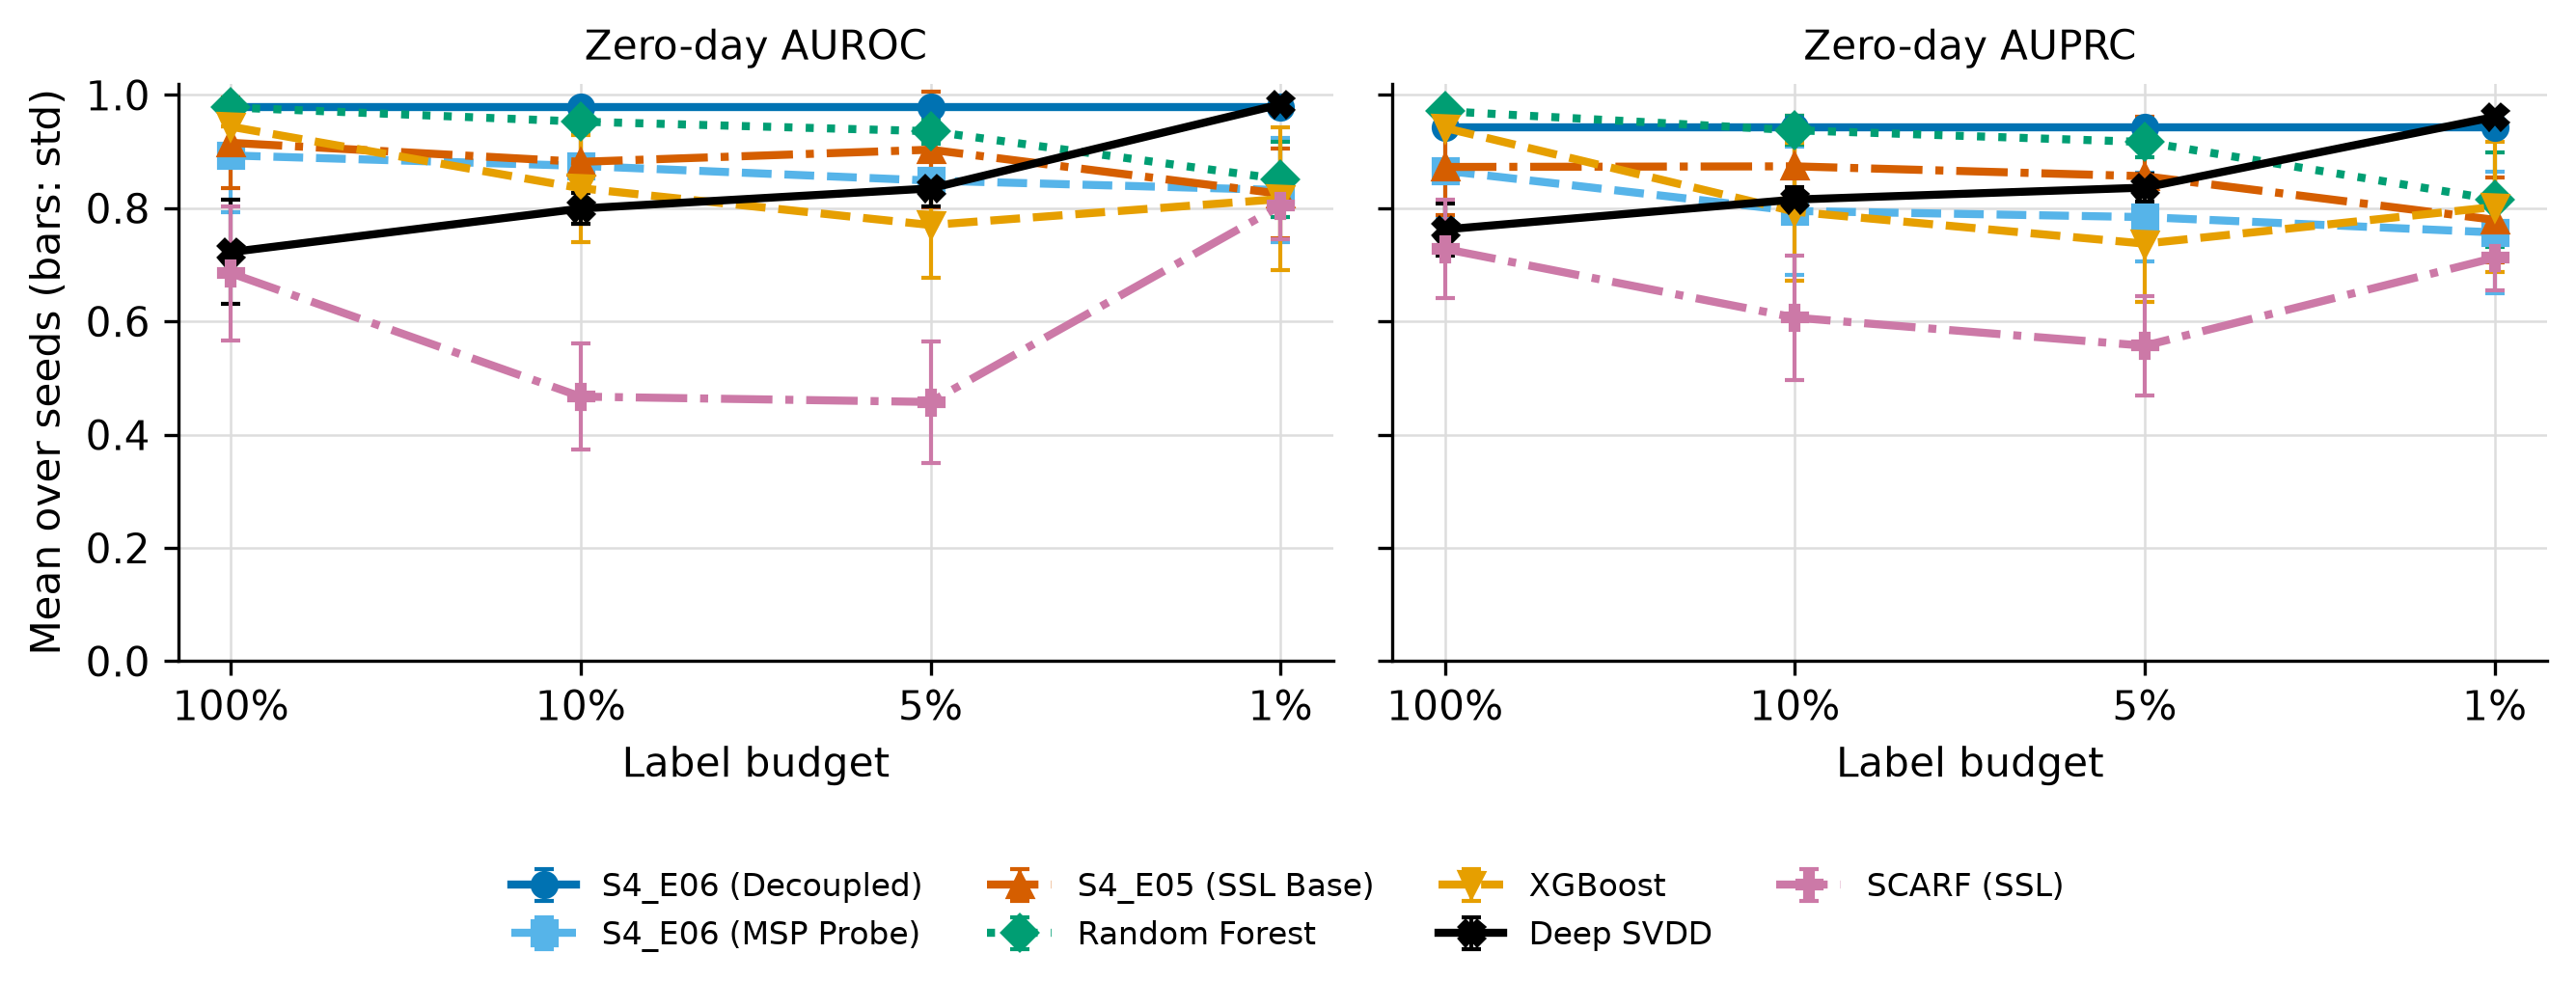
\includegraphics[width=\linewidth]{assets/fig_budget.png}
\captionof{figure}{Zero-day AUROC and AUPRC across label budgets (mean of 10 seeds; bars show one standard deviation).}
\end{center}
\begin{center}
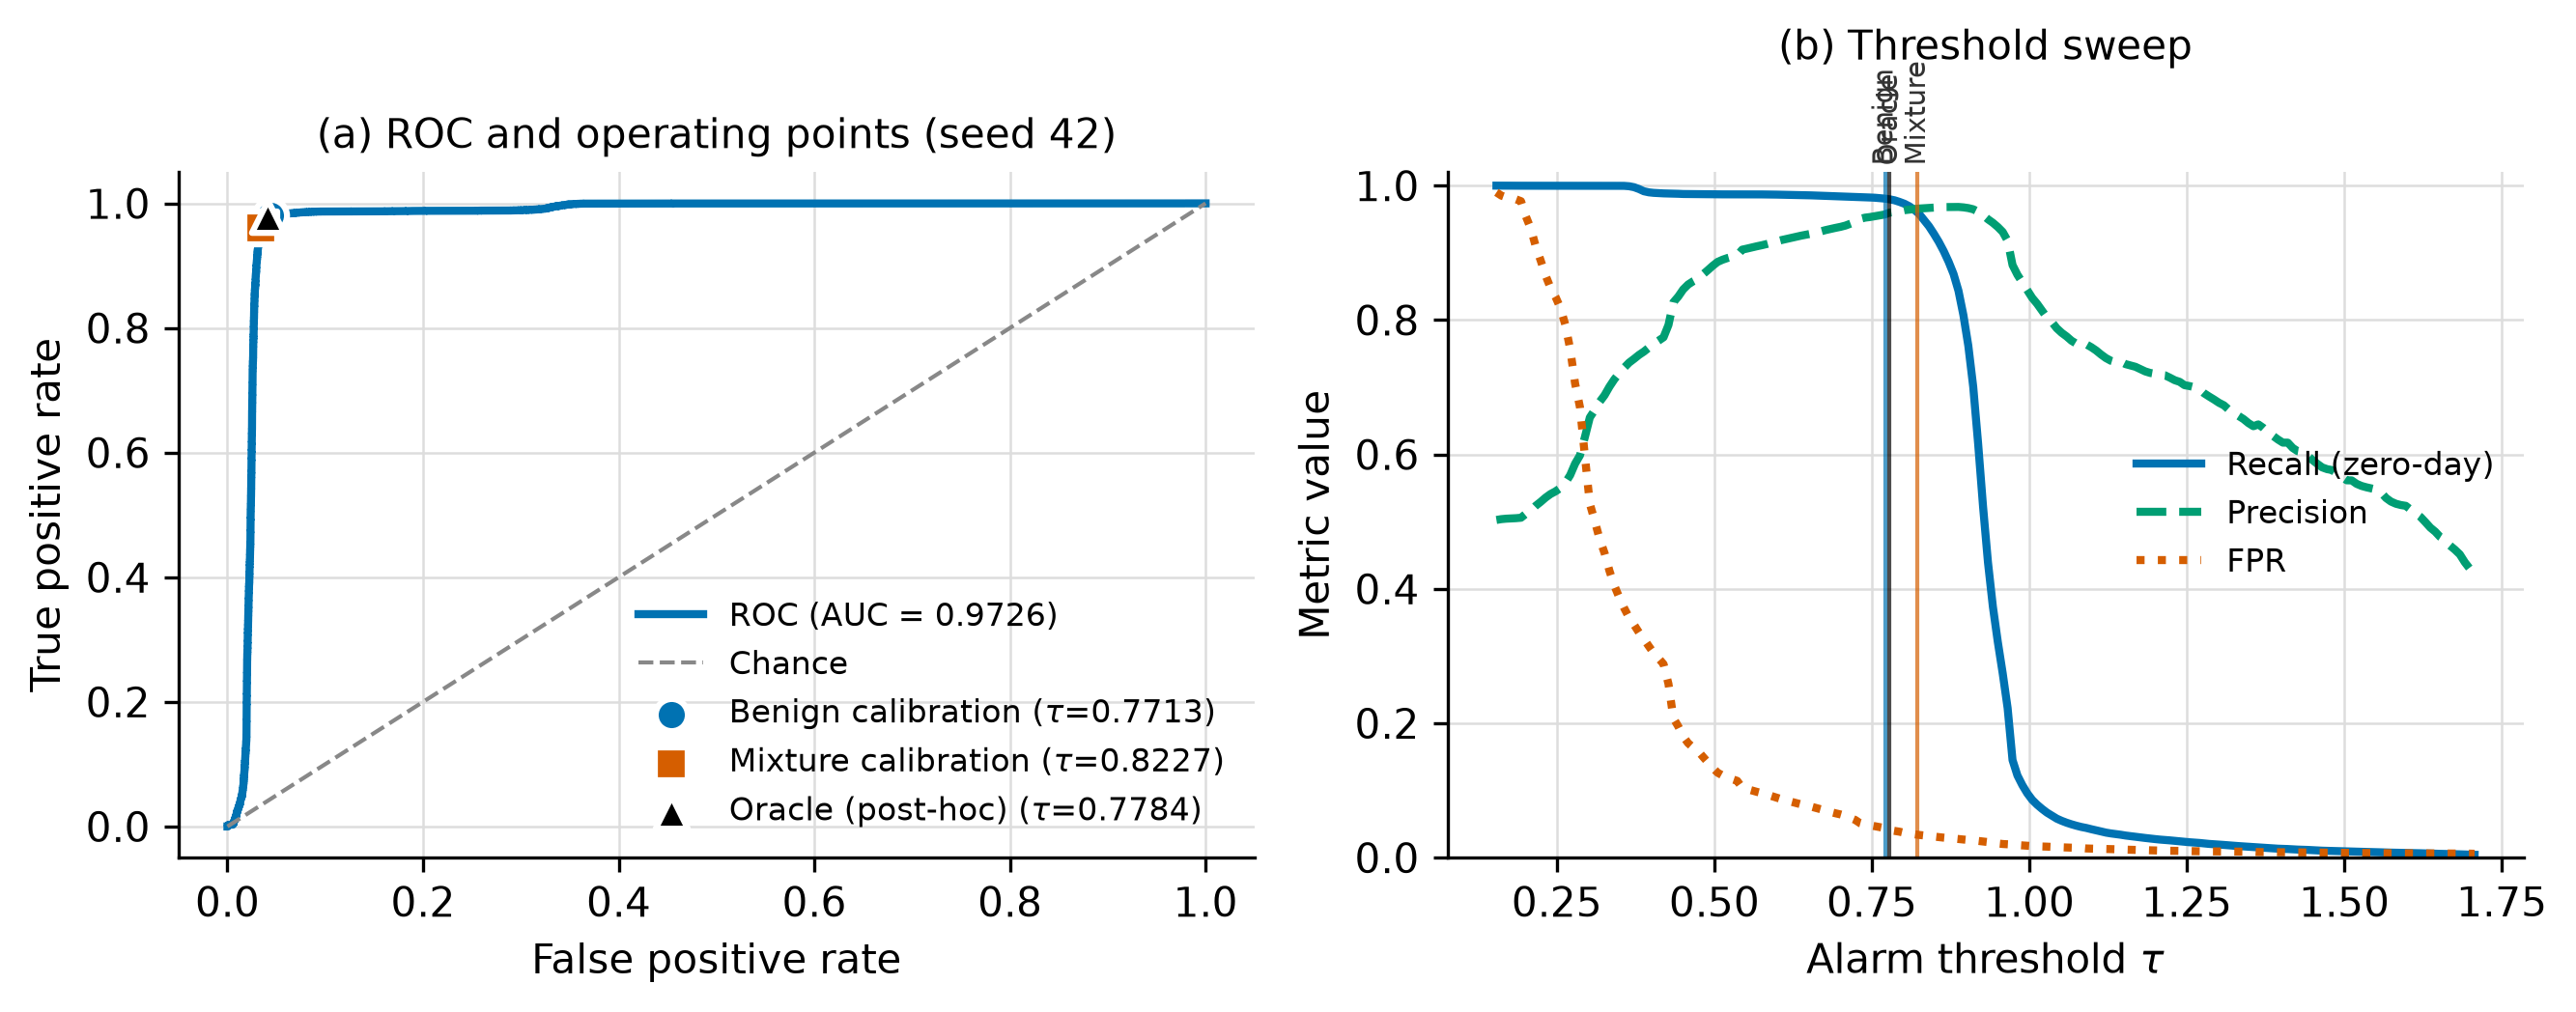
\includegraphics[width=\linewidth]{assets/fig_operating.png}
\captionof{figure}{Decoupled score on the locked test set, seed 42, 10\% labels. (a) ROC curve with the benign-calibrated, mixture-calibrated and post-hoc oracle operating points. (b) Recall, precision and false-positive rate against the threshold. The oracle point reads test labels and is a diagnostic only.}
\end{center}
\begin{center}
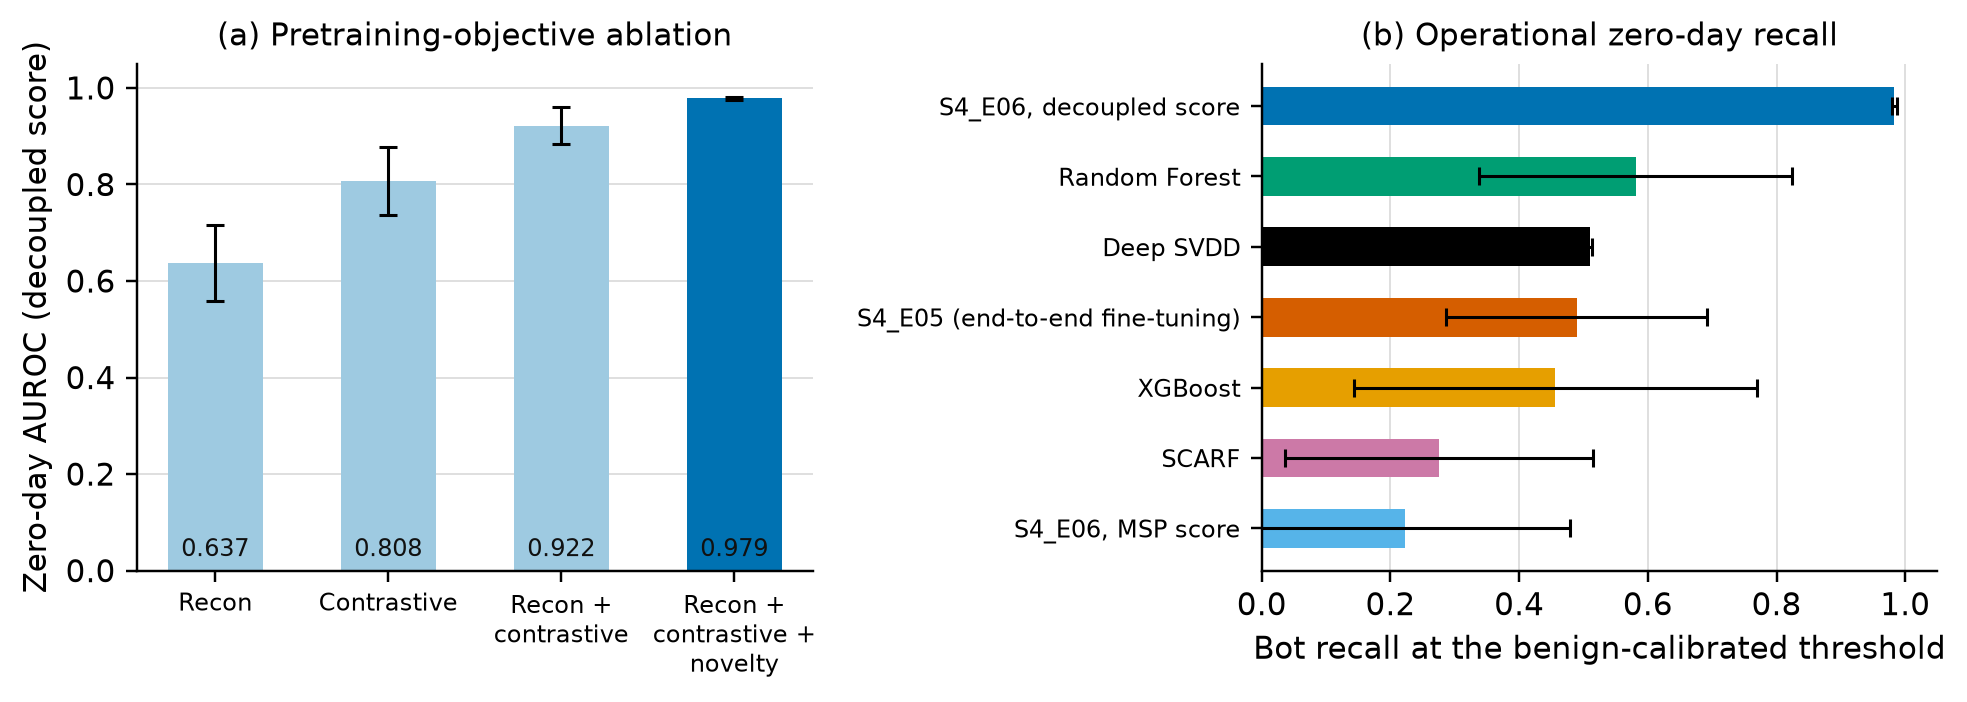
\includegraphics[width=\linewidth]{assets/fig_bars.png}
\captionof{figure}{(a) Decoupled AUROC for each combination of pretraining objectives. (b) Bot recall at the calibrated threshold for every model. Bars show one standard deviation over 10 seeds.}
\end{center}
\section{Component Ablation Study}
\subsection{Pretraining Objectives}
Each objective combination was pretrained for all ten seeds and evaluated with a frozen probe at the 10\% budget (Table 8). Each added objective raises the decoupled AUROC and narrows its spread. The novelty term has the opposite effect on MSP, whose AUROC falls when the latents are compacted. The two scores therefore favour different geometries, and the novelty term is useful only together with centroid scoring.

\begin{center}
\captionof{table}{Objective ablation, 10\% labels, 10 seeds.}
\begin{adjustbox}{max width=\linewidth}\small
\begin{tabular}{llll}
\toprule
{\bfseries\boldmath Pretraining objectives} & {\bfseries\boldmath Decoupled AUROC} & {\bfseries\boldmath Decoupled AUPRC} & {\bfseries\boldmath MSP AUROC} \\
\midrule
Reconstruction only & 0.6370 $\pm$ 0.0794 & 0.7309 $\pm$ 0.0413 & 0.9043 $\pm$ 0.1092 \\
Contrastive only & 0.8077 $\pm$ 0.0706 & 0.7208 $\pm$ 0.1020 & 0.8910 $\pm$ 0.0954 \\
Recon + Contrastive & 0.9216 $\pm$ 0.0384 & 0.8858 $\pm$ 0.0508 & 0.9437 $\pm$ 0.0468 \\
{\bfseries\boldmath Recon + Contrastive + Novelty} & {\bfseries\boldmath 0.9785 $\pm$ 0.0028} & {\bfseries\boldmath 0.9423 $\pm$ 0.0095} & {\bfseries\boldmath 0.8747 $\pm$ 0.0822} \\
\bottomrule
\end{tabular}
\end{adjustbox}
\end{center}
\subsection{Scoring Rules on the Same Encoder}
Table 9 applies eight scoring rules to the S4\_E06 encoder. The two centroid distances are equivalent and best. Mahalanobis and nearest-neighbour distances rank well but detect only about half of the Bot flows at the calibrated threshold. The last two rows apply the same reference-based rules to the scaled input features with no encoder; they fail on Bot, which shows that the learned representation, not the distance rule alone, carries the result.

\begin{center}
\captionof{table}{Zero-day scores computed on the S4\_E06 encoder, 10\% labels, 10 seeds.}
\begin{adjustbox}{max width=\linewidth}\small
\begin{tabular}{lllll}
\toprule
{\bfseries\boldmath Zero-day score} & {\bfseries\boldmath AUROC} & {\bfseries\boldmath AUPRC} & {\bfseries\boldmath Recall at $\tau$} & {\bfseries\boldmath FPR at $\tau$} \\
\midrule
{\bfseries\boldmath Distance to pool centroid (decoupled, proposed)} & {\bfseries\boldmath 0.9785 $\pm$ 0.0028} & {\bfseries\boldmath 0.9423 $\pm$ 0.0095} & {\bfseries\boldmath 0.9827 $\pm$ 0.0037} & {\bfseries\boldmath 0.0436 $\pm$ 0.0013} \\
Distance to benign centroid & 0.9784 $\pm$ 0.0035 & 0.9421 $\pm$ 0.0108 & 0.9837 $\pm$ 0.0022 & 0.0433 $\pm$ 0.0013 \\
Mahalanobis distance to benign & 0.9378 $\pm$ 0.0061 & 0.9120 $\pm$ 0.0084 & 0.5089 $\pm$ 0.0039 & 0.0518 $\pm$ 0.0016 \\
Class-conditional Mahalanobis & 0.9189 $\pm$ 0.0074 & 0.8938 $\pm$ 0.0100 & 0.5088 $\pm$ 0.0048 & 0.0527 $\pm$ 0.0020 \\
k-NN distance to benign & 0.9144 $\pm$ 0.0149 & 0.8896 $\pm$ 0.0142 & 0.5111 $\pm$ 0.0002 & 0.0507 $\pm$ 0.0015 \\
Maximum softmax probability & 0.8747 $\pm$ 0.0822 & 0.7950 $\pm$ 0.1136 & 0.2230 $\pm$ 0.2554 & 0.0451 $\pm$ 0.0172 \\
No encoder: k-NN distance to benign & 0.7434 $\pm$ 0.0191 & 0.6490 $\pm$ 0.0098 & 0.0034 $\pm$ 0.0004 & 0.0557 $\pm$ 0.0011 \\
No encoder: Mahalanobis to benign & 0.4214 $\pm$ 0.0088 & 0.4240 $\pm$ 0.0034 & 0.0037 $\pm$ 0.0000 & 0.0594 $\pm$ 0.0006 \\
\bottomrule
\end{tabular}
\end{adjustbox}
\end{center}
\section{Robustness Analysis}
\subsection{Stand-In Zero-Days}
To examine hyperparameters without touching the test day, one known attack class at a time was removed from training entirely and the model was scored on separating benign validation flows from that class. Four classes and two seeds were used. No pretraining setting improved on the stated configuration by more than about 0.01 on the benign-distance scores, and tripling the epochs did not help, so the stated configuration was kept (Table 10). Removing the novelty term lowers the decoupled score from 0.68 to 0.41.

\begin{center}
\captionof{table}{Mean AUROC over four stand-in zero-days and two seeds, by pretraining setting.}
\begin{adjustbox}{max width=\linewidth}\small
\begin{tabular}{llll}
\toprule
{\bfseries\boldmath Pretraining setting} & {\bfseries\boldmath Decoupled} & {\bfseries\boldmath k-NN to benign} & {\bfseries\boldmath Mahalanobis to benign} \\
\midrule
{\bfseries\boldmath Stated configuration (10 epochs, mask 0.2, $\lambda$\textsubscript{nov} 0.2)} & {\bfseries\boldmath 0.6821} & {\bfseries\boldmath 0.8335} & {\bfseries\boldmath 0.8285} \\
30 pretraining epochs & 0.5984 & 0.8295 & 0.8319 \\
Mask rate 0.4 & 0.6799 & 0.8355 & 0.8289 \\
Contrastive temperature 0.5 & 0.7012 & 0.8315 & 0.8233 \\
No input LayerNorm & 0.6457 & 0.8339 & 0.8269 \\
$\lambda$\textsubscript{nov} = 1.0 & 0.7100 & 0.8298 & 0.8298 \\
No novelty loss & 0.4101 & 0.8408 & 0.8361 \\
\bottomrule
\end{tabular}
\end{adjustbox}
\end{center}
Table 11 breaks the stated configuration down by held-out class. The decoupled score is uneven: it is near chance on Infiltration and moderate elsewhere, with a mean of 0.68. Benign-distance scores are steadier (mean 0.83), and on Slowloris a nearest-neighbour rule on raw features is as good as any learned score. Infiltration is hard for every score.

\begin{center}
\captionof{table}{AUROC on each stand-in zero-day for the stated configuration (mean of two seeds).}
\begin{adjustbox}{max width=\linewidth}\small
\begin{tabular}{llllll}
\toprule
{\bfseries\boldmath Zero-day score} & {\bfseries\boldmath DDoS LOIC-HTTP} & {\bfseries\boldmath DoS Slowloris} & {\bfseries\boldmath Infilteration} & {\bfseries\boldmath SSH-Bruteforce} & {\bfseries\boldmath Mean} \\
\midrule
Distance to pool centroid (decoupled, proposed) & 0.8025 & 0.7205 & 0.5058 & 0.6998 & 0.6821 \\
k-NN distance to benign & 0.9452 & 0.9351 & 0.5363 & 0.9175 & 0.8335 \\
Mahalanobis distance to benign & 0.9068 & 0.9509 & 0.5749 & 0.8813 & 0.8285 \\
Maximum softmax probability & 0.5857 & 0.6548 & 0.5585 & 0.6071 & 0.6015 \\
No encoder: k-NN distance to benign & 0.9230 & 0.9656 & 0.4997 & 0.8981 & 0.8216 \\
\bottomrule
\end{tabular}
\end{adjustbox}
\end{center}
\subsection{Transport Shortcut Check}
Random Forest was retrained with destination port and protocol restored. Its zero-day AUROC is 0.9523 $\pm$ 0.0112 with the identifiers and 0.9528 $\pm$ 0.0207 without them. No shortcut effect is present in this protocol.

\section{Computational Cost}
Table 12 reports medians over ten seeds at the 10\% budget on a Colab Tesla T4 with two CPU cores; tree models run on the CPU. Pretraining is a one-off cost per seed and is reused across budgets. Deployed inference for the proposed model is 0.56 ms per 1,000 flows. The trained model has 477,726 parameters, of which 325,718 are deployed.

\begin{center}
\captionof{table}{Model size and measured cost, 10\% labels.}
\begin{adjustbox}{max width=\linewidth}\small
\begin{tabular}{lllllll}
\toprule
{\bfseries\boldmath Model} & {\bfseries\boldmath Deployed size} & {\bfseries\boldmath Pretraining} & {\bfseries\boldmath Adaptation} & {\bfseries\boldmath Inference / 1,000 flows} & {\bfseries\boldmath Peak GPU memory} & {\bfseries\boldmath Checkpoint} \\
\midrule
S4\_E06 & 325,718 parameters & 34.6 s & 0.93 s & 0.56 ms & 274 MB & 1.31 MB \\
S4\_E05 (end-to-end fine-tuning) & 325,718 parameters & 32.8 s & 2.45 s & 0.46 ms & 267 MB & 1.31 MB \\
Random Forest & 100,953 tree nodes & --- & 2.80 s & 8.74 ms & CPU & 17.82 MB \\
XGBoost & 1,400 trees & --- & 6.22 s & 17.27 ms & CPU & 1.72 MB \\
Deep SVDD & 58,368 parameters & --- & 0.55 s & 0.09 ms & 153 MB & 0.24 MB \\
SCARF & 125,646 parameters & 13.5 s & 0.94 s & 0.17 ms & 273 MB & 0.51 MB \\
\bottomrule
\end{tabular}
\end{adjustbox}
\end{center}
\section{Discussion, Limitations \& Conclusion}
\subsection{Why Decoupling Helps}
The probe and the zero-day score read the same encoder, yet MSP reaches AUROC 0.8747 with a standard deviation of 0.0822 while centroid distance reaches 0.9785 with 0.0028. MSP depends on where the probe happens to place Bot flows among the known classes, which changes with the seed and the labelled subset. Centroid distance depends only on pretraining, which uses 160,526 unlabelled flows and is stable.

\subsection{Limitations}
\begin{itemize}
\item \textbf{One zero-day family.} The headline result is for Bot. On stand-in zero-days the decoupled score is much weaker, so the model should not be described as a general zero-day detector.
\item \textbf{Not best at every budget.} Random Forest matches it with all labels and Deep SVDD exceeds it with 1\%.
\item \textbf{Weaker triage.} Tree ensembles classify known attacks better at every budget.
\item \textbf{One dataset.} No cross-dataset transfer was evaluated.
\item \textbf{Balanced test set.} The test set is half Bot. At a realistic 1\% prevalence the precision of the calibrated operating point falls to about 18\% for seed 42.
\end{itemize}
\subsection{Conclusion}
Under a leakage-controlled chronological protocol, a self-supervised tabular encoder with decoupled centroid scoring detects the held-out Bot family more accurately and far more stably than five baselines when 5\% to 10\% of labels are available, while retaining multi-class triage. The ablation attributes the gain to the combination of the three pretraining objectives with centroid scoring. The stand-in analysis shows the gain is family-dependent, and tree ensembles remain the better classifiers of known attacks.

\vspace{4pt}\begin{center}\fbox{\begin{minipage}{0.95\linewidth}\small \textbf{Reproducibility.} Code, tests, configuration and all run outputs are at \href{https://github.com/AakashBhat1/zeroday-intrusion-detection-ssl}{github.com/AakashBhat1/zeroday-intrusion-detection-ssl}. Every number in this report is computed from \href{https://github.com/AakashBhat1/zeroday-intrusion-detection-ssl/blob/main/paper1_results/results/runs.jsonl}{\texttt{paper1\_results/results/runs.jsonl}} and \href{https://github.com/AakashBhat1/zeroday-intrusion-detection-ssl/blob/main/paper1_results/results/tune.jsonl}{\texttt{tune.jsonl}}; the tables are also in \href{https://github.com/AakashBhat1/zeroday-intrusion-detection-ssl/tree/main/paper1_results/report}{\texttt{paper1\_results/report/}}, the split manifest in \href{https://github.com/AakashBhat1/zeroday-intrusion-detection-ssl/blob/main/paper1_results/data/manifest.json}{\texttt{paper1\_results/data/manifest.json}}, and this report is generated by \href{https://github.com/AakashBhat1/zeroday-intrusion-detection-ssl/blob/main/tools/build_report.py}{\texttt{tools/build\_report.py}}. Dataset: CSE-CIC-IDS2018, public bucket \texttt{s3://cse-cic-ids2018}.\end{minipage}}\end{center}

\end{document}
